% !TEX root = ../paper.tex

\begin{center}
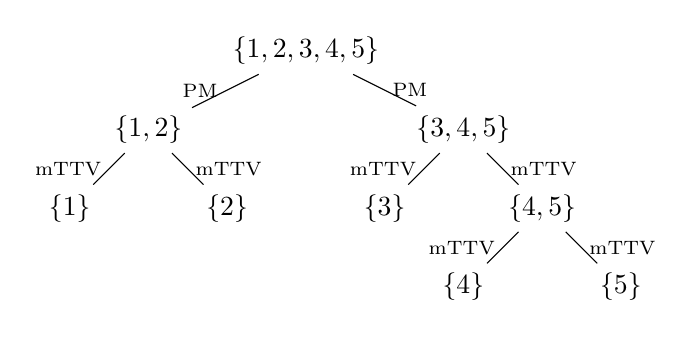
\begin{tikzpicture}

\node (12345) at (4,2) {$\{1,2,3,4,5\}$};
\node (12) at (2,1) {$\{1,2\}$};
\node (345) at (6,1) {$\{3,4,5\}$};
\node (1) at (1,0) {$\{1\}$};
\node (2) at (3,0) {$\{2\}$};
\node (3) at (5,0) {$\{3\}$};
\node (45) at (7,0) {$\{4,5\}$};
\node (4) at (6,-1) {$\{4\}$};
\node (5) at (8,-1) {$\{5\}$};

\scriptsize
\path[draw] (12345) edge [left,align=right] node {PM} (12);
\path[draw] (12345) edge [right,align=left] node {PM} (345);
\path[draw] (12) edge [left,align=right] node {mTTV} (1);
\path[draw] (12) edge [right,align=left] node {mTTV} (2);
\path[draw] (345) edge [left,align=right] node {mTTV} (3);
\path[draw] (345) edge [right,align=left] node {mTTV} (45);
\path[draw] (45) edge [left,align=right] node {mTTV} (4);
\path[draw] (45) edge [right,align=left] node {mTTV} (5);
\normalsize

\end{tikzpicture}
\end{center}